\documentclass{article}

\usepackage{graphicx}
\usepackage{tikz}
\usepackage{tikzsymbols}
\usetikzlibrary{calc,patterns,shapes.geometric}
\pagestyle{empty}
\usepackage[margin=0pt]{geometry}
\geometry{papersize={14in,12in}}

\def\centerarc[#1](#2)(#3:#4:#5){\draw[#1] ($(#2)+({#5*cos(#3)},{#5*sin(#3)})$) arc (#3:#4:#5);}

\begin{document}
	\begin{figure}
		\centering
		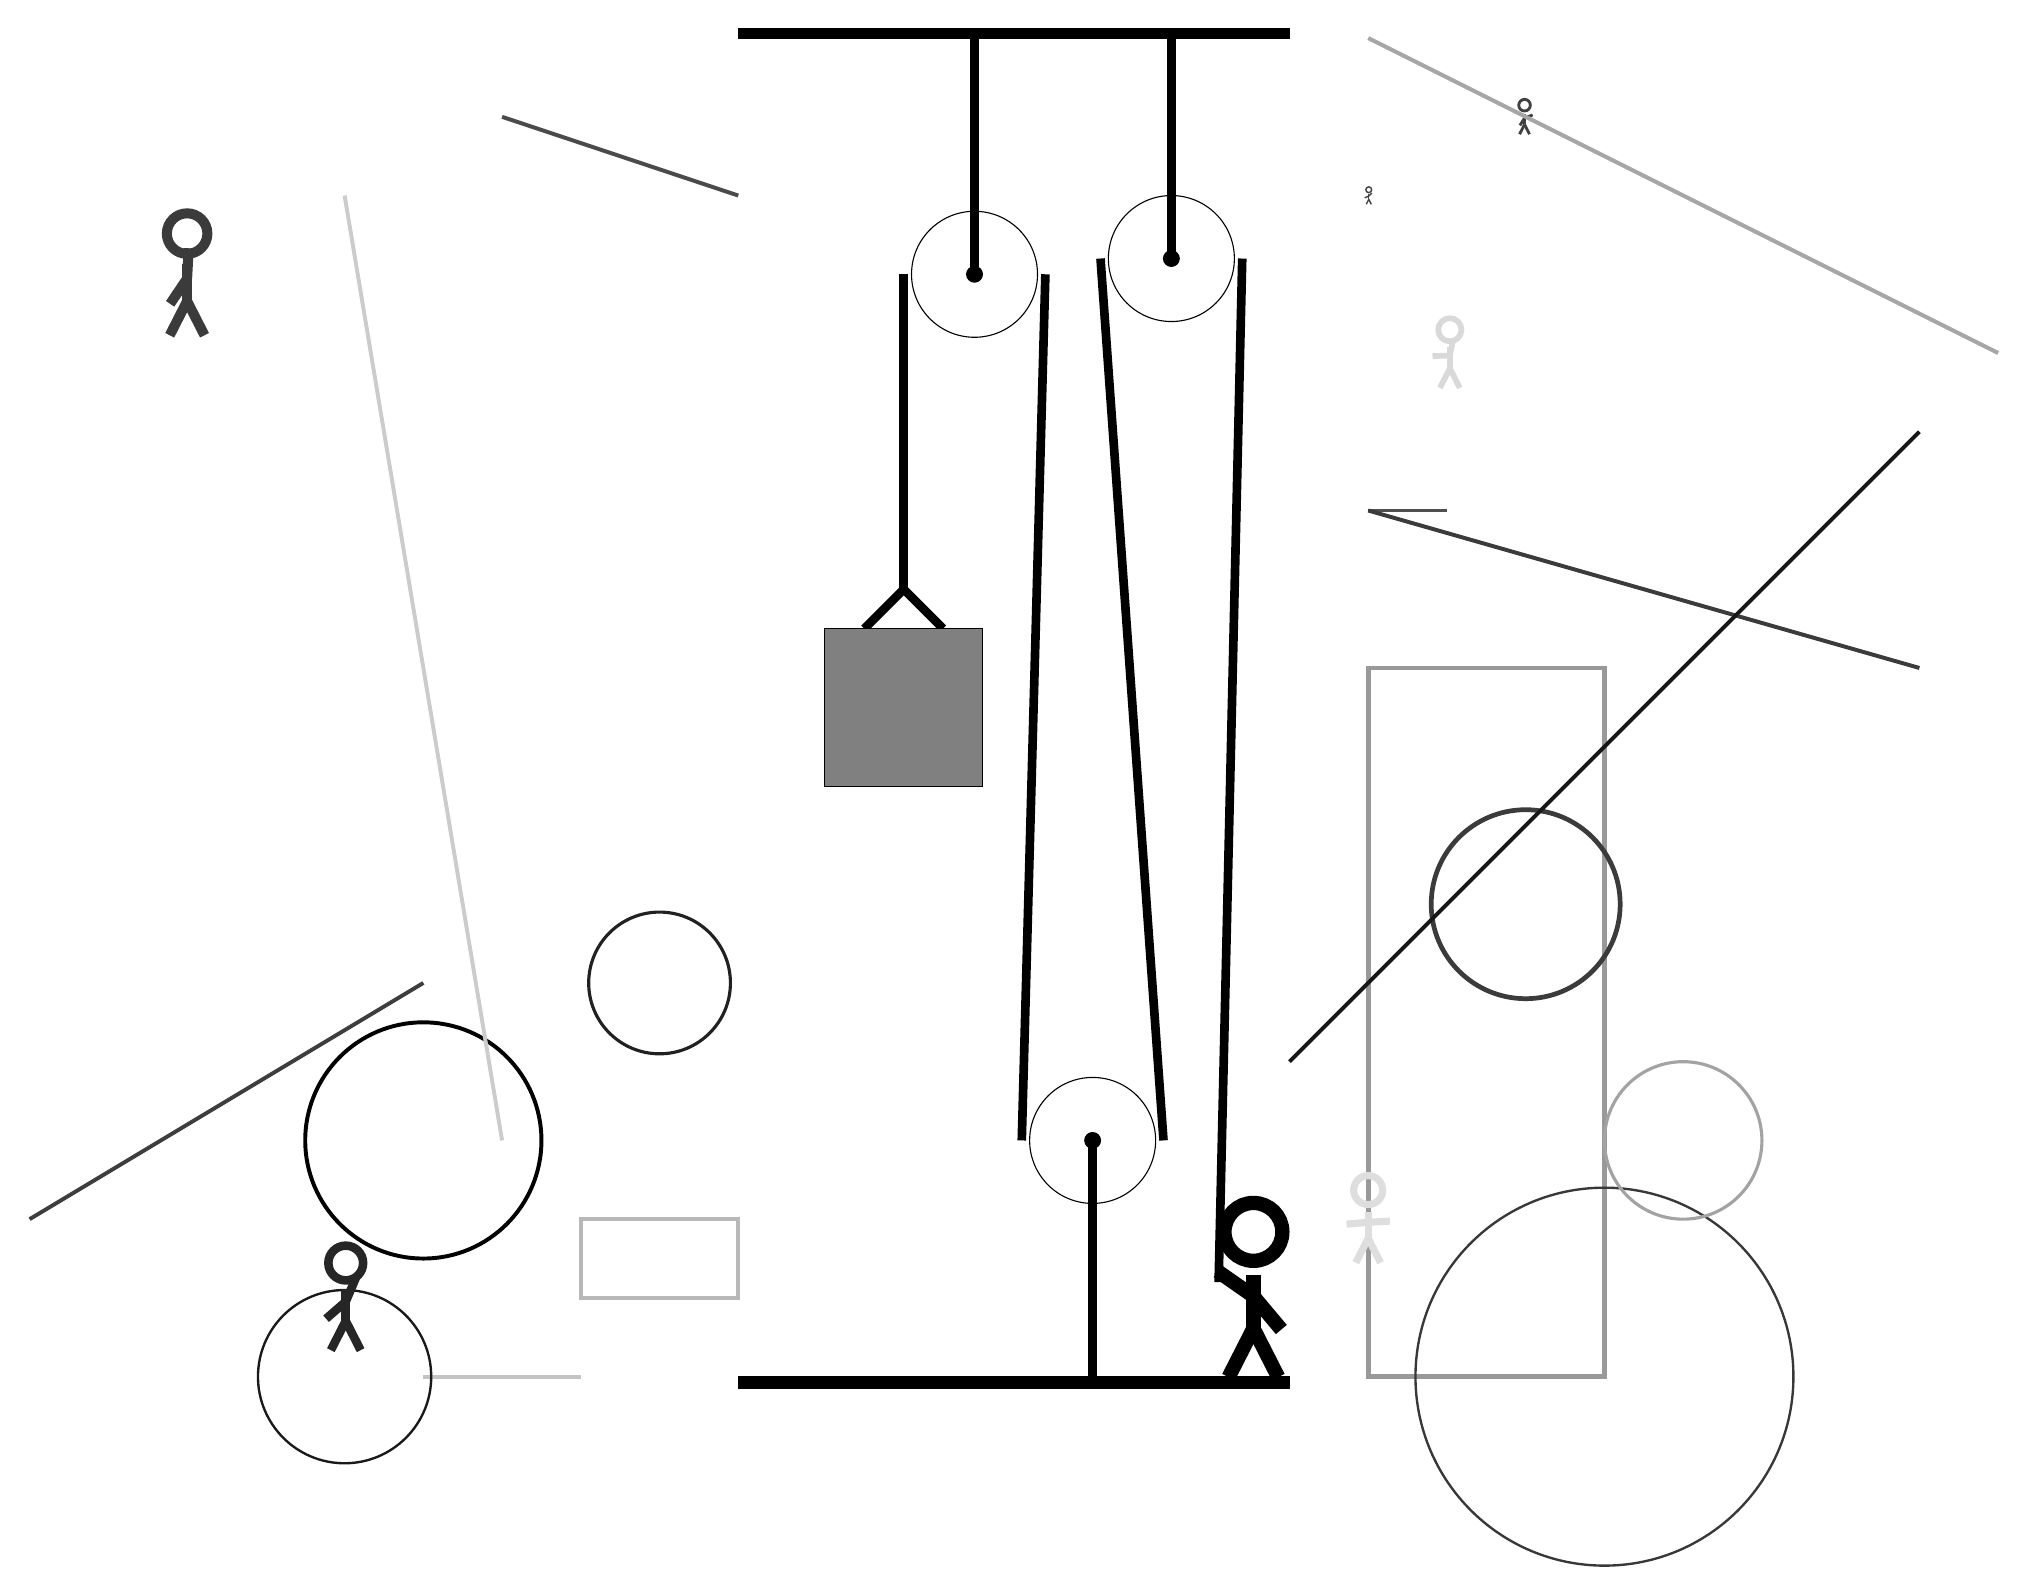
\begin{tikzpicture}
			%%%%% START %%%%%
			
			\draw[fill=black] (-2, 14) rectangle (5, 14.125);
			
			\draw (1, 11) circle (0.8);
			\draw[fill=black] (1, 11) circle (0.1);
			\draw[line width=1.1mm]  (1, 14) -- (1, 11);
			
			\draw[fill=white](2.5, 0) circle (0.8);
			\draw[fill=black] (2.5, 0) circle (0.1);
			\draw[line width=1.1mm]  (2.5, -3) -- (2.5, 0);
			
			\draw[fill=white](3.5, 11.2) circle (0.8);
			\draw[fill=black] (3.5, 11.2) circle (0.1);
			\draw[line width=1.1mm] (3.5, 14) -- (3.5, 11.2);
			
			\draw[line width=1.1mm] (-0.4, 6.5) -- (0.1, 7.0) -- (0.6, 6.5);
			\draw[fill=black!50] (-0.9, 6.5) rectangle (1.1, 4.5);
			
			\node[line width=0.4mm, color=black!77] at (-9, 11) {\Strichmaxerl[7][56][87]};
			
			\draw [line width=0.5mm, color=black!100](-6, 0) circle (1.5);
			\draw[line width=0.5mm, color=black!76](-6, 2) -- (-11, -1);
			\draw[line width=0.5mm, color=black!23](-6, -3) -- (-4, -3);
			
			\draw[line width=0.5mm, color=black!28] (-2, -2) rectangle (-4, -1);
			
			\draw[line width=0.6mm, color=black!40] (6, 6) rectangle (9, -3);
			
			\node[line width=0.3mm, color=black!75] at (8, 13) {\Strichmaxerl[2][58][21]};
			
			\draw[line width=0.5mm, color=black!20](-5, 0) -- (-7, 12);
			\draw [line width=0.3mm, color=black!90](-7, -3) circle (1.1);
			\draw[line width=0.3mm, color=black!69] (6, 8) rectangle (7, 8);
			
			\draw[line width=0.5mm, color=black!77](6, 8) -- (13, 6);
			
			\draw [line width=0.6mm, color=black!77](8, 3) circle (1.2);
			\draw [line width=0.3mm, color=black!78](9, -3) circle (2.4);
			\draw[line width=0.5mm, color=black!35](6, 14) -- (14, 10);
			\node[line width=0.7mm, color=black!13] at (6, -1) {\Strichmaxerl[5][5][3]};
			\draw[line width=0.5mm, color=black!71](-2, 12) -- (-5, 13);
			
			\node[line width=0.3mm, color=black!15] at (7, 10) {\Strichmaxerl[4][2][78]};
			
			\node[line width=0.7mm, color=black!74] at (6, 12) {\Strichmaxerl[1][21][47]};
			\draw [line width=0.4mm, color=black!36](10, 0) circle (1.0);
			\draw[line width=0.5mm, color=black!91](5, 1) -- (13, 9);
			\node[line width=0.5mm, color=black!85] at (-7, -2) {\Strichmaxerl[6][41][67]};
			\draw [line width=0.4mm, color=black!87](-3, 2) circle (0.9);
			
			
			\draw[line width=1.1mm] (0.1, 11) -- (0.1, 7.0);
			\centerarc[line width=1.1mm](1, 11)(0:180:0.9);
			\draw[line width=1.1mm](1.9, 11) -- (1.6, 0);
			\centerarc[line width=1.1mm](2.5, 0)(180:360:0.9);
			\draw[line width=1.1mm](3.4, 0) -- (2.6, 11.2);
			\centerarc[line width=1.1mm](3.5, 11.2)(0:180:0.9);
			\draw[line width=1.1mm](4.4, 11.2) -- (4.1, -1.8);
			
			\node at (4.5, -1.9) {\Strichmaxerl[10][-35][-50]};
			
			\draw[fill=black] (-2, -3) rectangle (5, -3.15);
			
			%%%%% END %%%%%
		\end{tikzpicture}
	\end{figure}	
\end{document}